%%%% ijcai17.tex

\typeout{IJCAI-17 Instructions for Authors}

% These are the instructions for authors for IJCAI-17.
% They are the same as the ones for IJCAI-11 with superficical wording
%   changes only.

\documentclass{article}
% The file ijcai17.sty is the style file for IJCAI-17 (same as ijcai07.sty).
\usepackage{ijcai17}

% Use the postscript times font!
\usepackage{times}
\usepackage{graphicx}
\usepackage{helvet}
\usepackage{courier}
\usepackage{epsfig}
\usepackage{amssymb}
\usepackage{amsmath}
\usepackage{amsfonts}
\usepackage{algorithm}
\usepackage{algorithmic}
\usepackage{mdwlist}
\usepackage{multirow}
\usepackage{color}
\usepackage{subfigure}
\usepackage{url}
\usepackage{enumerate}
\usepackage{threeparttable}

% the following package is optional:
%\usepackage{latexsym} 

% Following comment is from ijcai97-submit.tex:
% The preparation of these files was supported by Schlumberger Palo Alto
% Research, AT\&T Bell Laboratories, and Morgan Kaufmann Publishers.
% Shirley Jowell, of Morgan Kaufmann Publishers, and Peter F.
% Patel-Schneider, of AT\&T Bell Laboratories collaborated on their
% preparation.

% These instructions can be modified and used in other conferences as long
% as credit to the authors and supporting agencies is retained, this notice
% is not changed, and further modification or reuse is not restricted.
% Neither Shirley Jowell nor Peter F. Patel-Schneider can be listed as
% contacts for providing assistance without their prior permission.

% To use for other conferences, change references to files and the
% conference appropriate and use other authors, contacts, publishers, and
% organizations.
% Also change the deadline and address for returning papers and the length and
% page charge instructions.
% Put where the files are available in the appropriate places.

\title{Cascade Dynamics Modeling with Attention-based Recurrent Neural Network}
% \title{Recurrent Nerual Network Based On Attention Mechanism for Cascade
% Dynamics Modeling}
\author{}

\begin{document}

\maketitle

\begin{abstract}
Modeling the generation process of cascade has important implications for
understanding information propagation and launching viral marketing.
Majority of previous works focus on interpersonal influence modeling based on
diffusion models, limited by model bias and requirement of hidden diffusion
networks. Although traditional sequence modeling has no limitation on hidden
diffusion network, such modeling method can hardly exploit complex dependence
and propagation patterns. Therefore we apply RNN in cascade dynamics modeling.
We propose attenion-based RNN to solve crossing dependency problem, caused
by tree-structured propagations. Furthermore, we propose coverage in
attention-based RNN, leading the alignments focused more on recent propagations.
The experimental results demonstrate the effectiveness of our proposed model in
multiple prediction tasks and propagation structure inference.

\end{abstract}
\section{Introduction}

The emergence of Social Media platform has revolutionized dissemination of
information via its great ease in inforamtion delivery, accessing and filtering. 
In Social Media, pieces of information, posted by users spontaneously, propagate
along social relationships between users, explict or implict, forming cascade dynamics.
Modeling cascade dynamics is the fundamental to understand information
propagation and launch series of social applications, i.e., viral marketing,
popularity prediction and rumor detection. 

In order to model the cascades, many information diffusion models have been
proposed in the literature, such as discrete-time independent cascade model,
discrete-time linear threshold model and continuous-time independent cascade
model. A diffusion model is often associated with a directed graph and 
parameterized by propagation probabilities defined on edges or interpersonal
influence defined on nodes.
% interpersonal influence defined on edges or
% interactions between users. 
Kempe et al.~\cite{kempe2003maximizing} implemented
the linear threshold model by a degree-modulated edge weight. Goyal et
al.~\cite{goyal2010learning} provided two static models in terms of Bernoulli
distribution and Jaccard index, and learned temporal factors to maximize
likelihood of cascades. Gomez-Rodriguez et al.~\cite{gomez2013modeling}
estimated a transimission function over time associated with each edge, assuming
that observed diffusion time is independently sampled according to the
transimission function. Wang et.al~\cite{WangAAAI15}
captured users' influence and susceptibility in latent space and model the
transition probabilities of users' activated status according to users' latent
characteristics.

% survival model 
% and a
% cascade from a model is just a set of influenced nodes according to the model
% given a set of source nodes. 
% 
% The majority of works in cascade dynamics modeling is based on information
% diffusion models.
% 
% A diffusion model is often associated with a directed graph and a cascade from a
% model is just a set of influenced nodes according to the model given a set of
% source nodes. In gerneral, we have the following three typical types of
% diffusion models: discrete-time independent cascade model, discrete-time linear threshold
% model, continuous-time independent cascade model and 
% 
% The key to cascade dynamics modeling is to find a well-defined 
% function in hypothesis space based on observed cascades and forecast following
% propagations. Existed methods for this problem fall into two main paradigms:
% interpersonal influence modeling and sequential modeling. The majority of works
% focus on interpersonal influence modeling,  defining activation
% function on users, 

% The key to cascade dynamics modeling is to find a well-defined function in
% hypothesis space based on observed cascades. Existed methods for this problem
% fall into three main paradigms: pairwise, nodewise and eventwise modeling. The
% majority works in cascade dynamics modeling focus on pairwise modeling,
% defining the propagation probability of information between all pairs of
% users~\cite{SaitoPredDiffusionProb08,goyal2010learning,gomez2013modeling}.
% However, pairwise models suffer severe overfitting and overrepresentation
% problems especially in sparse social data, proved in \cite{WangAAAI15}.
% Nodewise modeling learn latent user-specific characteristics instead of pairwise
% manners, effectively combating overfitting and overrepresentation problems.
% Bourigault et.al.~\cite{bourigault2016representation} learn user-specific
% latent space in Independent Cascade (IC) model. Wang et.al~\cite{WangAAAI15}
% capture users' influence and susceptibility in latent space and define
% propagation probability according to users latent characteristics.
% Kurashima et.al.~\cite{KurashimaKDD14} embeded users into low-dimensional
% visualization space in Continous Time Independent Cascade (CTIC) model. But
% nodewise models require strong prior knowledge on generation processes of
% cascades in order to better fit the observations. Recently, eventwise models
% received great success in modeling sequence data. 

\begin{figure}[t]
\label{fig:mot}
\centering
\includegraphics[width=0.45\textwidth]{figs/mot.eps}
\caption{
An example of crossing dependency problem in sequence modeling. 
% Tree structure of propagation and crossing dependency problems in
% sequence modeling. For modeling dependence between 1st and 3rd event, we must
% use redundant information passing from 2nd event, called
% ``redundant modeling''. If we abandon useful information inherited by 3rd
% event when modeling the 4th event, the generation of 5th event would lose
% useful information from 3rd event, called ``cut-off modeling''.
}
\end{figure}

However, the information diffusion is too complicated to easily determine
the most appropriate diffusion model in practice. The misspecified diffusion
model would lead to large model bias. Besides, the diffusion network structure
can be also hidden from us. We need to learn the underlying
diffusion network structure with respect to parameter estimation in diffusion
model at most cases. It often leads to under-determined high computational cost
where specialized methods need to be designed. 

% Real world information diffusion is complicated, and it is not easy to determine
% the most suitable diffusion model in practice. A chosen diffusion model may be
% misspecified compared to real world data and lead to large model bias. 
% 
% The diffusion network structure can be also hidden from us, so we need to learn
% not only the paramters in the diffusion model, but also the diffusion network
% structure. This often leads to under-determined high dimensional estimation
% problem where specialized methods need to be designed. 

Instead of learning a particular diffusion model, sequence modeling can be
used to discover complex dependencies and patterns between the following
propagation and current histories, thus modeling the cascade dyanmics.
For example, Manavoglue~\cite{Manavoglu2003userbehaviormodels} proposed a user
behavior generation method based on maxent and Markov mixture model. Recently,
the efficient way of sequence modeling can be achieved by Recurrent Neural
Network
(RNN)~\cite{goldberg2014word2vec,mikolov2010recurrent,sundermeyer2012lstm}.
Du et al.~\cite{DuKDD2016} proposed a RNN framework, called RMTPP,
where the embedding of hidden units are used to parameterize the generation
process of propagations. The benefits of sequence modeling are two-fold: 1)
It avoids strong prior knowledge on diffusion model; 2) It has no limitation on
hidden social network structure. 

% The benefits of eventwise modeling are
% two folds: 1) avoiding strong prior knowledge on models and networks with
% respect to different observed cascades; 2) enlarging the functional space when
% searching the optimal cascade dynamics models, which may have great probability
% to better model cascade dynamics. 
% 
% Eventwise methods aims to
% learn history embedding in order to model the generation of next event, e.g., cascade. 
% Manavoglu~\cite{Manavoglu2003userbehaviormodels} propose users behavior
% generation method based on maxent and Markov mixture model. Recently, the
% efficient way of eventwise modeling can be achieved by Recurrent Neural Network
% (RNN)~\cite{bengio2003neural,goldberg2014word2vec,mikolov2010recurrent,sundermeyer2012lstm}.
% Du et.al.~\cite{DuKDD2016} proposed a Recurrent Marked Temporal Point Process
% (RMTPP) for event streams. The outputs of hidden layer in Recurrent Neural
% Network (RNN) represents the embedding of the event histories,
% then parameterizing the random process. The benefits of eventwise modeling are
% two folds: 1) avoiding strong prior knowledge on models and networks with
% respect to different observed cascades; 2) enlarging the functional space when
% searching the optimal cascade dynamics models, which may have great probability
% to better model cascade dynamics. 

Despite of advantages in sequence modeling, the traditional methods
may meet ``crossing dependency'' problem in cascade dynamics modeling, mainly
caused by
%  The crossing dependencies problem is mainly caused by 
tree structure of propagation. Fig.~\ref{fig:mot} shows the crossing
dependency dilemma in practical. 
As consideration
of tree strucutre of propagations, we need to construct the dependence between
the 1st and the 3rd propagations, causing redundant information usage passing
from the 2nd one (the transitive dependence marked as grey in time
line). If we abandon information inherited from the 2nd propagation, the
generation of 4th propagation will lose useful information from the 2nd
one as the corresponding user $u_4$ is directly connected to $u_2$ on the
cascade tree
(the transitive dependence marked as red in time line). 
% For modeling the dependence between the 1st
% and 3rd propagation, we must use redundant information passing from the 2nd
% one.
% % , called ``redundant modeling''. 
% Otherwise, if we abandon useful information inherited from the 2nd propagatoin,
% the generation of the 4th propagation will lose some useful information as the
% corresponding user $u_4$ is directly connected to $u_2$ on the cascade tree.
% event when modeling the 4th event, the generation of 5th event would lose
% useful information from 3rd event, called ``cut-off modeling''. Crossing
% dependency problems limit the efficiency of sequence modeling.
In this paper, we propose a \textbf{C}ascade d\textbf{Y}namics
modeling with \textbf{A}ttentio\textbf{N}-based RNN (CYAN-RNN) to better
apply RNN in cascade dynamics modeling. We construct a dynamic pooling
layer above hidden units of RNN, aggregating all embeddings of hidden units
until current step. The generation of following propagation is relied on the
aggregated embedding. 
% The weights in pooling layer pointing to each historical event
% embedding refers to connections between current event and history. 
We choose attention mechanism~\cite{bahdanau2014neural} to realize the pooling layer,
where the parameters can be automatically learned by maximizing the
likelihood of cascade. 
% The benifits of our proposed model are three-fold: 
More specifically, our work makes the following contributions:
\begin{itemize}
  \item We exploit crossing dependency problem existed in traditional sequence
  modeling when applied to model cascade dynamics and proposed attention-based
  RNN to solve the problem;
  \item We propose attention mechansim with coverage to further improve the
  performance of attention mechanism;
  \item The alignments in proposed attention mechanism are homologous to the
  underlying structure of propagation.
\end{itemize}
% 1) We exploit crossing dependency problem existed in traditional sequence
% modeling when applied to model cascade dynamics and proposed attention-based 
% RNN to solve the problem;
% We propose two sequence modeling methods based on RNN for cascade dyanmics
% modeling;
% eventwise method, using sequence
% modeling, for cascade dynamics modeling; 
% 2) We propose attention mechansim with coverage to further improve the
% performance of attention mechanism;
% 3) The alignments in proposed attention mechanism are homologous to the
% underlying structure of propagation.   
% 
% We exploit crossing dependency problem existed in traditional sequence
% modeling when applied to cascade dynamics modeling. The alignments in
% proposed attention mechanism can 
% 
% point out crossing dependency problem in
% traditional sequence modeling when model cascade dynamics. Thus, we
% proposed CYAN-RNN to solve the problem; 
We conduct extensive experiments on synthetic
and real-world datasets. Compared with several widely-used methods in cascade
dynamics modeling, our proposed models consistently outperform them at
predicting next propagations. 

% we exploit quantitative analysis to
% understand 
% the experimental results show that our model consistently
% outperform than previous modeling methods in cascade dynamics modeling.

% to limit hypothesis space 
% 
% require strong prior knowledge on generation of cascade data in
% order to determine specific form of cascade model as the limitation of
% hypothesis space.

% To overcome the drawbacks in pairwise modeling, n
% 
% Nodewise modeling and
% eventwise modeling.
% 
% Existed methods for this problem
% fall into three main paradigms. 

% In Social Media, users can post  information spontaneously, spreading 
% 
% The emergence of Social Media platform has motivated a large mount of
% hot researches, including Social Network Analysis, Marketing and Information
% Propagation. 

\section{Model}

\subsection{Background}
% \noindent{\textbf{CDM based on RNN:}}
Firstly, we introduce RNN as an eventwise modeling method in cascade dynamics
modeling. A cascade $S=\{x_i|x_i=(t_i, u_i), u_i\in U \text{~and~}
t_i\in R^+\}_{i=1}^N$ is a set of propagations asendingly ordered by time,
where $U$ refers to all possible users in cascades. The $i$-th propagation $x_i$
is recorded as a tuple $(t_i, u_i)$ referring to activated time and activated user
respectively. At each step $k$, the $k$-th propagation are fed into hidden
units by nonlinear transformation $f$, jointly with the outputs from the
previous hidden units, updating the hidden state $h_k=f(x_i,h_{k-1})$. The
representation of hidden state $h_k$ can be considered as event embedding to
the $k$-th propagation~\cite{DuKDD2016}, and the output is trained to predict
the next propagation $x_{k+1}$ given $h_k$. In other words, we use RNN to
maximize the likelihood probability of observed propagations,
\begin{equation}
\label{eq:likelihood}
p(\textbf{x})=\prod_{k=1}^N p(x_{k+1}|h_k)
\end{equation}
% The embeddings of propagations $E(x_i)$ are given as inputs
% to RNN. At each step $k$, the network updates its hidden state $h_k=f(E(x_i),
% h_{k-1})$, where $f$ is certain nonlinear functions.  
% In RNN, the input to an encoder is an activation sequence
% $S=\{x_i|x_i=(t_i, u_i)\}_{i=1}^N$ asendingly ordered by time. The activation
% $x_i$ is recorded as a tuple $(t_i, e_i)$ referring to activated time and activated
% user respectively. The embeddings of activation are given as inputs to RNN. At
% each step $k$, the network updates 
% The current inputs are fed
% into hidden units by nonlinear transformation, jointly with the outputs from the
% previous hidden units, and then generate the next activation in cascade. The
% representation of hidden units can be recognized as the event embedding
% to the corresponding inputs. 
Based on sufficient observed cascades, RNN
can find an optimal solution for Eq.~(\ref{eq:likelihood})
in a huge functional space, avoiding the limits of prior knowledge. Thus, RNN
can be a promising method to capture the complex propagation patterns in cascade
dynamics modeling. 

However, RNN suffers crossing dependency problem caused by tree structure
propagations in cascade, shown in Fig.~\ref{fig:mot}. One of the possible
solutions is to construct a pooling layer above the hidden
units in order to build the direct dependency between the generation of $k$-th
propagation and all previous event embeddings, i.e.,
$p(x_{k+1} | \text{pooling}(h_1,\ldots,h_k))$. The simplest way of pooling can
be formalized as
\begin{equation}
\label{eq:pooling_frame}
s_k=\sum_{i=1}^k \alpha_{k,i} h_i \text{,~~~~~s.t.~} \sum_{i=1}^k
\alpha_{k,i}=1,
\end{equation}
where the weight $\alpha_{k,i}$ refers to the proportion of dependency between
next propagation and the $i$-th event embedding. Mean pooling and max pooling
are two popular choices for setting weights which takes the mean or element-wise
max of all hidden states. However, these two methods still ignore the structure
information in cascades.
% Mean pooling and max pooling
% are two popular choices for setting weights which takes the mean or
% element-wise max of all hidden states. 
% In this way, the generation of next activation
% can depend on any historical embedding instead of transitive dependency.
Intuitively, the weights can be settled according to the cascade tree, yet we
can hardly observe the tree structure even given the social relationships. Next
we propose attention mechanism to implement the pooling layer. 

\subsection{CYAN-RNN}
Attention mechanism is orginally used in neural machine translation (NMT),
firstly proposed by Bahdanau et.al~\cite{bahdanau2014neural}. In the
senario of attention-based NMT, the target words are translated by the words in
source sequence and attention mechanism can automatically learn the alignment
between source words and target words~\cite{}.
% the words in source sequence need to be
% aligned to the words in target sequence. 
% Attention-based RNN can adaptively
% learn the alignment between source and target sequences. 
However, there are two
problems when applying attention mechanism in cascade dyanmics modeling: 1)
only one single sequence can be observed in a cascade; 2) the size of alignments
in attention mechanism need to be updated when the context $\{h_1,\ldots,h_k\}$
is growing along with the proceeding propagations.

\begin{figure}[t]
\centering
\includegraphics[width=0.45\textwidth]{figs/cyanrnn_framework.png}
\caption{The architecture of CYAN-RNN. The figure presents the case when
predicting the $(k+1)$-th propagation. The sequence in bottom is the observed
cascade and the sequence in top is the cascade shifted one step
according to the observation. The blue rectangles refer to representations from
the hidden units in source sequence, attention layer, and hidden units in
target sequence. The yellow rectangle is a component functioned in neural
network.}
\label{fig:cyrnn_frame}
\end{figure}

Thus, we propose CYAN-RNN for cascade dynamics modeling, applying a dynamic
attention mechanism to solve the crossing dependency problem. The architecture
of CYAN-RNN is shown in Fig.~\ref{fig:cyrnn_frame}. In CYAN-RNN, we conduct the
observed cascade as the source sequence. The target sequence is the copy of
source sequence, shifting one step of the copy backwards. The objective is to
jointly predict the next propagation and learn the alignment of dependency
between the next propagation and histories. 
% As to the target
% sequence, we copy the source sequence and then shift one step of the copy backwards. 
According to the architecture, we define each conditional probability in
Eq.~(\ref{eq:likelihood}) as:
\begin{equation}
\label{eq:cond_prob}
p(x_{k+1}|x_1,\ldots,x_k)=g(x_k, t_{k}, s_{k}),
\end{equation}
where $g$ is an objective function defined the joint probability of
propagation on activated user and activated time. Here we use the objective function
defined on RMTPP~\cite{DuKDD2016}.
% \begin{equation}
% \label{eq:rmtpp}
% \begin{aligned}
% g(x_k,t_{k},s_{k})&=p(u_{k+1}|t_k, s_k, x_k)\cdot p(t_{k+1}| t_k, s_k, x_k)\\
% &=\text{softmax}(t_k, s_k, x_k)\cdot
% \lambda(t_{k+1})\exp\left(-\int_{t_k}^{t_{k+1}}\lambda(\tau)d\tau \right)
% \end{aligned}
% \end{equation}
The $t_k$ is a hidden state related
to the $k$-th step of target sequence, computed by
\begin{equation}
\label{eq:target_embedding}
t_k = f(x_k, t_{k-1}, s_k),
\end{equation}
where 
% subscript in exponential function is the index of vector.   
$f$ is
a nonlinear activation function, which can be either a \textit{tanh} or
\textit{sigmoid} function. The context vector $s_k$ is calculated by
Eq.~(\ref{eq:pooling_frame}) where the weights $\alpha_{k,.}$ 
% in proposed attention mechanism 
is updated by the growth context
$\{h_1,\ldots,h_k\}$ and $t_{k-1}$. We can get the weights
\begin{equation}
\label{eq:alpha}
\alpha_{k,i}=\frac{\exp(e_{k,i})}{\sum_{j=1}^k \exp(e_{k,j})},
\end{equation}
where
\begin{equation}
\label{eq:score}
e_{k,i}=a(t_{k-1}, h_i)=v^T\tanh(W t_{k-1}+U h_i)
\end{equation}
scores how well the dependency between the $i$-th event
embedding and the output at the $k$-th step. The implementation of attention
mechanism in proposed model is briefly represented in Fig.~\ref{fig:att}. 

Given a collection of cascades $\mathcal{C}=\{S_m\}_{m=1}^M$, we suppose that
each cascade is independent on each other. As a result, the logarithmic
likelihood of a set of cascades is the sum of logarithmic likelihood of individual cascade.
In this way, the negative logarithmic likelihood of the set of cascades can be
estimated as
\begin{equation}
\mathcal{L}(\mathcal{C})=-\sum_{m=1}^M \sum_{k=1}^{N_m} \left[
g(x_k^{(m)}, t_{k}^{(m)}, s_{k}^{(m)}) \right], 
\end{equation}
and we can learn parameters of the proposed model by minimizing the negative
logarithmic likelihood.
%  $\arg \min_\theta \mathcal{L}(\mathcal{C})$, where $\theta$ is the
% parameter set in the model. 
With the attention mechanism, the alignment
weigts $\alpha_{k,.}$ can be directly updated through the cost function, thus
exploit an expected representation $s_k$ over all historic event embeddings for
each step $k$.

% The weights in proposed attention
% mechanism $s_k=\sum_{i=1}^k \alpha_i h_i$   
% The context vector $s_k$ is a representation, calculated in
% Eq.~(\ref{eq:pooling_frame}).

% to model cascade dynamics, the learned weights in
% attention and also infer the tree structure of propagations. The architecture of CYAN-RNN is shown in
% Fig.~\ref{fig:framework}.
% We firstly conduct the observed cascade as the source sequence.
% Then we copy the cascade and then shift one step of the copy backwards as the target
% sequence. 
 
\begin{figure}[ht!]
\centering
\subfigure[] {
\label{fig:att}
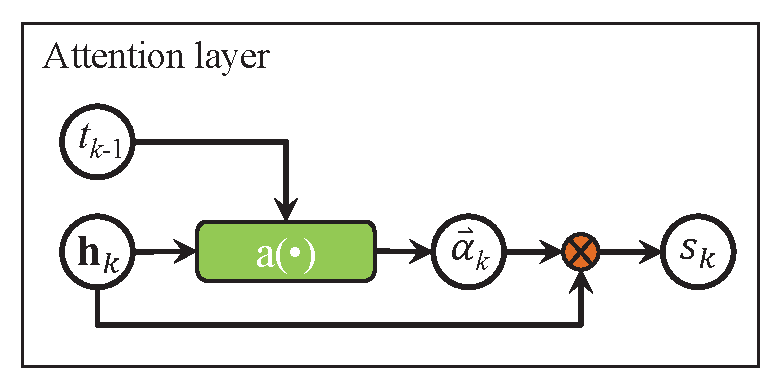
\includegraphics[width=0.35\textwidth]{figs/att.eps}
}
\subfigure[] {
\label{fig:cov}
\includegraphics[width=0.35\textwidth]{figs/cov.eps}
}
\caption{Two kinds of implementation on attention. (a) Attention mechanism
applied in CYAN-RNN; (b) Attention mechanism with coverage applied in CYAN-RNN
(cov). Note that $\textbf{h}_k=(h_1,\ldots,h_k)$ is matrix assembled by all
historic event embeddings at step $k$ and $\textbf{v}_k=(v_1,\ldots,v_k)$ is
a coverage martix containing all $k$-th coverage vectors.}
\end{figure}

\subsection{CYAN-RNN with Coverage}
\label{sec:coverage}

Although CYAN-RNN is proposed to better model cascade dynamics in consideration
of crossing dependency problem, the proposed model still suffer
\emph{over-dependent} and \emph{under-dependent} problems when applying
attention mechanism.
As the exmaple shown in Fig.~\ref{fig:mot}, if the user $u_1$ is an influential
user and his propagation is key to the cascade, the propagation activated by
$u_4$ may perfer to depend more on embedding of $(t_1, u_1)$ instead of $(t_2, u_2)$.
Here embedding of $(t_1, u_1)$ is over-dependent and embedding of $(t_2, u_2)$
is under-dependent. In practice, it is a common phenomenon that users may have a
higher probability activated by recent propagation than past ones~\cite{} and we
also conduct experiments to illustrate it (see section~\ref{sec:exp}).

The two problems are caused by memoryless of dynamic attention mechanism.
Inspired by linguistic coverage model~\cite{tu2016modeling}, we formulate the
general form of coverage, keeping historical alignments so
as to release the over-dependent and under-dependent problems. The $k$-th step
of coverage is defined as
\begin{equation}
\label{eq:cov}
V_{k,i}=f\left(V_{k-1, i}, \alpha_{k-1,i}, t_{k-1}, h_i\right).
\end{equation}
Remarkably, as the increasing propagations and alignments, $V_{k,k}$ and
$\alpha_{k,k}$ have no corresponding values in $V_{k-1,.}$ and
$\alpha_{k-1,.}$. Thus, we fill up with zeros in our works. 
Compared with $V_{k,i}$, $V_{k-1,i}$ 
At each step $k$, the $k$-th coverage serves an additional input to the
attention mechanism, providing complementary information of that how about the
dependencies of historical event embeddings are in the past. The rewritten
alignment calculation in Eq.~(\ref{eq:score}) by coverage can be
formalized~\footnote{The formalization is determined by the incremental length
of alignment weights. If we use the last coverage $V_{k-1,.}$ instead of
$V_{k,.}$ (like~\cite{tu2016modeling}) to update $e_{k,.}$ at each $k$
step, we will lose certain coverage information and cause unbalance
calculation about $k$-th event embedding, proved by our preliminary experiments.} as
\begin{equation}
\label{eq:att_cov}
\begin{aligned}
e_{k,i} &= a(t_{k-1}, h_i, V_{k,i}) \\
& = v^T\tanh(W t_{k-1}+U h_i+Z V_{k,i}).
\end{aligned}
\end{equation}
We expect that the alignment weights would be focus more on recent event
embeddings. The expectation will be validated in section~\ref{sec:exp}.   

\subsection{Window Size}
Practically, a cascade may last long and the propagation length would be huge,
causing an extreme computation cost when applying dynamic attention mechanism
proposed in CYAN-RNN. According to perference of users interests on recent
propagations, we consider a hyper-parameter, symboled by \emph{window size}
$l$, limiting the size of alignments so that the predicted task would only depend on
last $l$ propagations. Empirically, we set $l=200$ in most cases.

% Thus, the attention mechanism only need to calculate the
% $\max (k, t)$ historical event embeddings 

\section{Optimization}

In this section, we introduce the learning process of CYAN-RNN. 
The $k$-th propagation are transformed into vectors as inputs including user
embedding and temporal features. The user embedding matrix related to activated
users is learned along with the training process. The temporal features
related to activated time are formalized, inlcuding logarithm time interval
$\log(t_k-t_{k-1})$ and discretization of numerical attributes on year, month,
day, week, hour, mininute and second. We adopt
GRU~\cite{chung2014empirical} to encode the inputs of source sequence to event
embeddings $h$. We apply back-propagation through time
(BPTT)~\cite{chauvin1995backpropagation} for parameter estimation. The
parameters are iteratively updated by Adam~\cite{kingma2015method}, an
efficient stochastic optimization algorithm with mini-batch techniques. We also
employ early stopping method~\cite{prechelt1998automatic} to prevent
overfitting. The stopping criterion is achieved when the performance has no
more improvement in validation set. For speeding up the convergence, we use
orthogonal initialization method~\cite{henaff2016orthogonal} in training
process.

\section{Experiments}
\label{sec:exp}
In experiments, we compare our CYAN-RNN 
to the state-of-the-art modeling methods of cascade prediction on both
synthetic and real data. 
The results show that CYAN-RNN can better model cascade dynamics
and infer propagation structure.

\subsection{Baselines}
% We choose Recurrent Marked Temporal Point Process (RMTPP)~\cite{DuKDD2016} as
% one of the baselines which can models both next activated user and time based on
% RNN.
% \begin{itemize}
%   \item \textbf{RMTPP}~\cite{DuKDD2016}: Recurrent marked temporal point process
%   (RMTPP) is a method which can models both next activated user and time based on RNN.
% \end{itemize}
% However, only RMTPP~\cite{DuKDD2016} can predict next propagations completely
% including both next actived user and time. To better illustrate the performance of our
% proposed model, we choose other state-of-the-art models for either predicting
% next activated users or predicting next activated time for comparisons in two
% prediction tasks.

Rare methods can predict next propagations completely including both next
activated users and time. To better illustrate the performance of our
proposed model, we choose the state-of-the-art modeling methods for either
predicting next activated users or predicting next activated time for comparisons in two
prediction tasks.

(1) Prediction of next activated user
\begin{itemize}
  \item \textbf{CT Bernoulli} and \textbf{CT Jaccard}
  models~\cite{goyal2010learning}: They are continuous time propagation models.
  The propagation probabilities between two users are defined by Bernoulli or
  Jaccard distribution and the probabilities are decayed over time.
  \item \textbf{MC-1} Model: The markov chain model is a classic sequence
  modeling method. Here we compare with markov chain with order one.
\end{itemize}

(2) Prediction of next activated time 
\begin{itemize}
  \item \textbf{Poisson process} model~\cite{vere1988introduction}: It is a
  stoachastic point process model, depicting the time consuming from one
  propagation to another. The intensity function is parameterized by a constant.
  \item \textbf{Hawkes process} model~\cite{hawkes1971spectra}: It is a
  stochastic point process model where the intensity function is parameterized by
  \begin{equation} 
  \label{eq:hawke_intens_func}
  \lambda(t)=\lambda(0)+\alpha\sum_{t_i<t}\exp\left(-\frac{t-t_i}{\sigma}\right),
  \end{equation}
  where $\sigma=1$ and $\lambda(0)$ is a intrinsic rate when $t=0$.
\end{itemize}

We also compare with the model that has the ability to generate both mark and
temporal sequences.
\begin{itemize}
  \item \textbf{RMTPP}~\cite{DuKDD2016}: Recurrent marked temporal point process
  (RMTPP) is a method which can models both next activated user and time based on RNN.
\end{itemize}

\subsection{Synthetic Data and Results Anlaysis}
The goal of the experiments on synthetic
data is to understand how the underlying network structure and propagation
model affect our proposed model on both cascade prediction and
dependency structure inference. 

\noindent{\textbf{Data generation}} 
We use Kroneck
generator~\cite{LeskovecICML07} to construct two types of networks with directed
edges: 1) the Core-Periphery (CP) network~\cite{LeskovecWWW08} (Kroneck
parameter matrix $[0.962, 0.535; 0.535, 0.107]$), mimicing real-world social networks; 2) the
Erd\H{o}s-R{\'e}nyi random (Random) network~\cite{Erdos60} ($[0.5, 0.5; 0.5, 0.5]$). The incubation time
of one user activating anther user are sampled from the two distributions: 1)
mixed exponential (Exp) distributions, controlled by rate parameters $\alpha$
in $[0.01, 10]$; 2) mixed rayleigh (Ray) distribution, controlled
by scale parameters $\beta$ in $[0.01, 10]$. To generate a
cascade, we randomly choose a root user as the source of the cascade at first.
For each neighbor of the activated user, its activated time is determined by
incubation time. The propagation process will further conitune  in
breadth-first fashion until the overall time exceed the predefined observation
time window or no new user being activated. In our experiments, we set the total
number of users $|U|=32$ and the maximal observation time $\max\{t\}=100$.
As a result, four kinds of datasets are obtained by the different unions between
network and cascade generation distribution, denoted by (CP, Exp), (CP, Ray),
(Random, Exp) and (Random, Ray). We generate up to
20,000 cascades in each dataset, where we randomly pick up 80\% of completed sequences for training and the rest are
 evenly split into validation and test sets. 
% The policy of seperating dataset is uniform in real data.

\begin{figure*}[ht!]
\centering
\subfigure[CP, Exp] {
\label{fig:pred_usr_toy_cp_exp}
\includegraphics[width=0.235\textwidth]{figs/toy_mrr-cp-exp.png}
}
\subfigure[CP, Rayleign] {
\label{fig:pred_usr_toy_cp_ray}
\includegraphics[width=0.235\textwidth]{figs/toy_mrr-cp-ray.png}
}
\subfigure[Random, Exp] {
\label{fig:pred_usr_toy_rand_exp}
\includegraphics[width=0.235\textwidth]{figs/toy_mrr-rand-exp.png}
}
\subfigure[Random, Rayleign] {
\label{fig:pred_usr_toy_rand_ray}
\includegraphics[width=0.235\textwidth]{figs/toy_mrr-rand-ray.png}
}
\subfigure[RMSE on toy data] {
\label{fig:pred_tm_toy_rmse}
\includegraphics[width=0.235\textwidth]{figs/toy_rmse.png}
}
\subfigure[Real data] {
\label{fig:pred_usr_real}
\includegraphics[width=0.235\textwidth]{figs/real_mrr.png}
}
\subfigure[RMSE on real data] {
\label{fig:pred_tm_real_rmse}
\includegraphics[width=0.235\textwidth]{figs/real_rmse.png}
}

\caption{Comparisons on baselines and our proposed models. (a)$\sim$(e) The
predictions of next activated user and time on toy data produced
from different networks and propagation models; (f) and (g) The predictions of
next activated user and time on real data.}
\end{figure*}

%\noindent{\textbf{Evaluation metrics}} 
We regard the prediction task on next activated user as a ranking problem
with respect to transition probabilities. The predictive performance is
evaluated by \textit{Accuracy on top} $k$ (Acc@$k$) and \textit{Mean Reciprocal Rank}
(MRR)~\cite{voorhees1999trec}.
% , functionized in top $k$ and global perspectives.
The larger values in Acc@$k$ and MRR indicate the better performance.
On the prediction of next activated time, we use Root Mean Square Deviation
(RMSE) between estimated time and practical occuring time. The better
performance means the small values in RMSE.   

\noindent{\textbf{Prediction results.}} 
We regard the prediction task on next activated user as a ranking problem
with respect to transition probabilities. The predictive performance is
evaluated by \textit{Accuracy on top} $k$ (Acc@$k$) and \textit{Mean Reciprocal Rank}
(MRR)~\cite{voorhees1999trec}.
% , functionized in top $k$ and global perspectives.
The larger values in Acc@$k$ and MRR indicate the better performance.
On the prediction of next activated time, we use Root Mean Square Deviation
(RMSE) between estimated time and practical occuring time. The better
performance means the small values in RMSE.   

We conduct experiments on all four
kinds of datasets. 
We firstly compare the predictive preformance on
next activated users. The results on predictions of next
activated users are shown in Fig.~\ref{fig:pred_usr_toy_cp_exp}$\sim$
\ref{fig:pred_usr_toy_rand_ray}. As shown in the figures, CYAN-RNN and CYAN-RNN(cov)
perform consistently and significantly better than other baselines in metrics of
Acc@1, Acc@5 and MRR, included in all datasets. 
% In Acc@10, our proposed models
% outperform other baselines except the cases in dataset of
% (Random, Exp). 
% Despite of this, 
The results indicate that our proposed methods can better predict next activated
users. It is interested that RMTPP has lower accuracy or MRR values than CT Bern
and CT Jac in some cases shown in
Fig.~\ref{fig:pred_usr_toy_cp_ray},
\ref{fig:pred_usr_toy_rand_exp} and \ref{fig:pred_usr_toy_rand_ray}, however,
CYAN-RNN and CYAN-RNN(cov) can still performs better. It clearly demonstrates
that the proposed attention mechanism has the ability to directly capture past
propagation information which may be ``forgetten'' by sequential transitions in
RNN, called crossing dependency problems in CDM.
% Interestingly, we can find out that the RMTPP has lower accurary or MRR
% values in datasets of (CP, Rayleign), (Random, Exp) and (Random, Rayleign).
Fig.~\ref{fig:pred_tm_toy_rmse} compares the predictive performance on RMSE.
We can observe that Poisson and Hawkes processes are the worst modeling methods,
obtaining the errors larger than 2 hours in all datasets. Meanwhile, the
RMSE values are similar between RMTPP and CYAN-RNN. But 
CYAN-RNN(cov) can perform slightly better than RMTPP and CYAN-RNN in all
datasets when predicting next activated time. 
Additionally, we can observe that CYAN-RNN(cov) consistently perform better or
even than CYAN-RNN in two prediction tasks. It indicates that the coverage can
help to efficiently utilize the propagation embeddings in attention mechanism.
Next we will exploit the answers how the coverage can help to boost predictive
performance and lead to better inference on dependency structure.

\begin{figure}
\centering
\subfigure[] {
\label{fig:cyan_deps}
\includegraphics[width=0.225\textwidth]{figs/case_align-att.png}
}
\subfigure[] {
\label{fig:cyan_cov_deps}
\includegraphics[width=0.225\textwidth]{figs/case_align-cov.png}
}
\caption{Sample alignments on a fragement of cascade. The y-axis is the users
who will be activated next sequentiallly from top to bottom. The x-axis is the
activated order related to next activated user in the cascade. Each pixel shows
the weight $\alpha_{k,i}$ related to $i$-th propagation embedding at each step
$k$, in grayscale (0:black, 1:white). (a) the alignments inferred by CYAN-RNN; (b) the
alignments inferred by CYAN-RNN(cov).
% the inferred Graphs of
% propagations inferred by proposed models.
% The grey lines are the ground truth of propagation paths, while the read lines are wrong
% estimations, including missing or false answers. (a) Graph of propagation
% inferred by CYAN-RNN; (b) Graph of propagation inferred by CYAN-RNN (cov). 
}
\end{figure}

\noindent{\textbf{Alignment accurary.}} 
We expect to check if coverage can reduce the over-dependence and
under-dependence mentioned in section~\ref{sec:coverage}.
Fig.~\ref{fig:cyan_deps} and \ref{fig:cyan_cov_deps} show the results. Every grid
in each plot represents the alignment weights associated with propagation
embeddings.
The brighter grid refers to the larger weights corresponding to next
propagation. From this we see which positions in the past propagations
were considered more important when predicting next propagation. Comparing to
the alignments in CYAN-RNN, we can observe that the alignments in CYAN-RNN(cov)
concentrate more on unused propagation embeddings, which is consistent to
well-studied phenomonen in published works~\cite{}. Moreover, we wonder if the
inferred alignments is homologous to true propagation structures. Thus, we
calculate alignments on each step of cascades in test data. We suggest that the
propagation structure of next propagation can be inferred by the largest
alignment at each step. We then get a matrix of statistic results based on all inferred
structures. Every column in the matrix refers to the number of who mainly
activate the propagation. As the high connection between propagation
structure and network, the inferred structures would be the edges in
network. Therefore, we normalize the matrix by rows, and check if the
network edges can be classified by the matrix. As the
inference results are same in other two datasets, we only show the AUC values
computed by the models trained in dataset of (CP, Exp) and (Random, Exp),
decribed in Table~\ref{t:auc_net_inf}. The results from our proposed models
are both worked in network inference. Besides, CYAN-RNN(cov) obtain better results of
network inference than CYAN-RNN in two test data. It indicates that our
proposed alignment mechanism can be natually used in inference of hidden
propagation structure, which may have some potential applications in practice,
e.g., advertisement and recommendation.

%  to specific user. normalized
% normalize the  and treat the ms into a classification task.
% We suppose that the
% next propagation is only related to corresponding historical propagation which
% has the largest alignment weight. As the reason of relationship
% between propagation structures and network, we expect the connection between
% next propagation and corresponding 


\begin{table}[h!]
\centering
\caption{AUC values of network inference.}
\begin{tabular*}{.38\textwidth}{c|cc} \hline
Network & CYAN-RNN & CYAN-RNN(cov) \\ \hline
CP & 0.83 & 0.84 \\
Random & 0.95 & 0.96 \\ \hline
\end{tabular*}
\label{t:auc_net_inf}
\end{table}

% \begin{table}[h]
% \centering
% \caption{Distribution of dependency on relative position (inferred vs. ground
% truth).}
% \resizebox{0.47\textwidth}{!}{
% \begin{tabular}{crcc|c} \hline
% & & CYAN-RNN & CYAN-RNN(cov) & Ground truth \\ \hline 
% \multirow{5}{*}{CP} & 1st pos & 0.005 & & 0.022 \\
%  & last pos & 0.930 & 0 & 0.326 \\
%  & 1st prev pos & 0.065 & 0.968 & 0.182 \\
%  & 2nd prev pos & 0.004 & 0.032 & 0.121 \\
%  & 3rd prev pos & 0.002 & 0 & 0.087 \\ \hline
% \multirow{5}{*}{ER} & 1st pos &  & & 0.024 \\
%  & last pos pos & & & 0.387 \\
%  & 1st prev pos & & & 0.189 \\
%  & 2nd prev pos & & & 0.118 \\
%  & 3rd prev pos & & & 0.078 \\ \hline
% \end{tabular}
% }
% \end{table}

% \noindent{\textbf{Case study: alignment quality.}}

% CP, Exp(att, cov)
% Area under the ROC curve : 0.831982
% Area under the ROC curve : 0.839126
% Random, Exp(att, cov)
% Area under the ROC curve : 0.955918
% Area under the ROC curve : 0.956609

\subsection{Real Data and Result Analysis}

\noindent{\textbf{Experimental setup.}}  
The real data is extracted from Sina Weibo, a Chinese microblogging website,
spanning from June 1st, 2016 to June 30th, 2016. We focus the records in June
1st and extract users whose posting numbers are ranged in $(100,
200]$. Then we sort records according to the root
message IDs posted by the filtered users in 30 days and arrange them ascendingly
by posting time. We drop the cascades that the number of propagations is larger
than 1,000. The long length of propagations may dominate the training process,
however, rarely occurred in practice. 
%  thus ignoring the small ones.
Finally, the processed data contains 2964 users and 596,088 cascades. 
% The average number of users postings is up to 9581.76.
We use 536,240 sequences for training, 29,758 for validation and 30,005 for
testing. The task is to predict next propagation, including activated user and
time. 

\noindent{\textbf{Prediction results.}} 
The results on predictions of next
activate users and time are shown in Fig.~\ref{fig:pred_usr_real} and
\ref{fig:pred_tm_real_rmse}. The hyper-parameters of CYAN-RNN and CYAN-RNN(cov)
are setted up as following: learning rate is 0.0001; hidden layer size of
encoder is 20; hidden layer size of decoder is 10; window size is 200; coverage
size is 10; and batch size is 128. Note that we have no social
network in extracted real data, thus we cannot compare our proposed models with
CT Bern and CT Jac. CYAN-RNN and CYAN-RNN(cov) outperform the other baselines
with higher MRR values and lower RMSE values for predicting both next activated
users and time. Comparing to RMTPP, CYAN-RNN(cov) recieves 6.25\%, 5.48\% and
3.90\% relative increased performance on Acc@1, Acc@5 and MRR respectively, and
reduces 0.78\% relative errors on RMSE. Comparing to CYAN-RNN, CYAN-RNN(cov)
recieves 4.62\%, 2.67\% and 1.27\% relative increased performance on Acc@1,
Acc@5 and MRR respectively, and reduces 0.33\% relative errors on RMSE.

% \begin{figure}[ht!]
% \centering
% \subfigure[] {
% \label{fig:pred_usr_real}
% \includegraphics[width=0.35\textwidth]{figs/toy_mrr.png}
% }
% \subfigure[] {
% \label{fig:pred_tm_real}
% \includegraphics[width=0.35\textwidth]{figs/toy_rmse.png}
% }
% \caption{The next activated user and time predictions on real data. (a) The
% performance of predictions on next activated users related to baselines and our
% proposed models; (b) The performance of predictions on next activated time
% related to baselines and our proposed models.}
% \end{figure}

% \noindent{\textbf{Visualization.}} 

% \input{5-related.tex}
\section{Conclusion}

In this paper, we present the cascade dynamics modeling with attention-based
RNN. As we know, it is a prior attempt on CDM based on RNN, which embed
historical propagations into vectors and then determine the next propagation sequentially. 
Instead of traditional interpersonal influence modeling, RNN can
be used to discover complex dependencies and patterns between the following
propagation and current histories. 
% Instead of traditional interpersonal influence modeling, sequential modeling can
% be used to discover dependencies and patterns between the following propagation and
% current histories. 
However, RNN suffers crossing dependency problem when applying
in CDM. To solve the problem, we propose attention mechanism
above hidden units of RNN, named CYAN-RNN, aggregating all current historical
embeddings. Thus, the generation of next propagation can directly depend on all
current histories instead of transitive dependent way. Moreover, we propose
CYAN-RNN(cov) to construct coverage on attention mechanism in order to solve
over-dependent and under-dependent problem existed in CYAN-RNN. In experiments,
we evaluate the effectiveness of our proposed model on both synthetic and real
datasets. Experimental results demonstrate that our proposed models can
consistently outperform compared modeling methods at both predicition tasks of
next activated user and time. Addtionallly, CYAN-RNN(cov) performs
better or even than CYAN-RNN on both synthetic and real datasets, proving that
coverage can help to efficiently utilize historical embeddings in attention
mechanism. Besides, we conduct experiments to exploit alignment quality. The
results show that the alignments from our proposed models can reflect
true propagation structures, which may be well applicable in practice.

% have some potential applications in
% practice.
% four synthetic datasets
% produced from different networks and propagation models and one real dataset. 
% crossing-dependency way. We propose CYAN-RNN 
% 
% Based on RNN, the proposed model can embed historical propagations
% into vectors and the next propagation 


% \appendix

\newpage

%% The file named.bst is a bibliography style file for BibTeX 0.99c
\bibliographystyle{named}
\bibliography{/home/yqwang/Documents/bibtex/social}

\end{document}

